\RequirePackage{fix-cm}
\RequirePackage{amsmath} % solve problem with redefining \vec
%
%\documentclass{svjour3}                     % onecolumn (standard format)
%\documentclass[smallcondensed]{svjour3}     % onecolumn (ditto)
%\documentclass[smallextended]{svjour3}       % onecolumn (second format)
%\documentclass[twocolumn]{svjour3}          % twocolumn
%

%\documentclass[smallextended, draft]{svjour3}
\documentclass[smallextended]{svjour3}


\smartqed  % flush right qed marks, e.g. at end of proof
%
\usepackage{graphicx}
\usepackage{xcolor}
\usepackage{url}
\usepackage{hyperref}
\makeatletter
\renewcommand*{\eqref}[1]{%
  \hyperref[{#1}]{\textup{\tagform@{\ref*{#1}}}}%
}
\makeatother

% \usepackage{mathptmx}      % use Times fonts if available on your TeX system
%
% insert here the call for the packages your document requires
%\usepackage{latexsym}
% etc.

%%%%%%%%%%%%%%%%%% my personal header %%%%%%%%%%%%%%%%%%%
\usepackage{natbib} % for \citet and \citep

\usepackage{lineno}
\linenumbers

% \usepackage{makecell} % for multiple lines withinin one cell
% \usepackage{booktabs} % for more space between rows in a table
% \usepackage[flushleft]{threeparttable} % for also including table notes

\usepackage{sidecap}
\usepackage{hyperref}
\usepackage{caption}

\usepackage{amsfonts}
\usepackage{amssymb}
% \usepackage{amsmath}

\usepackage{enumerate}
%\usepackage{bm} % for bold vectors \bm{v}
\usepackage{bbm} % indicator function \mathbbm{1}
%\usepackage{pdflscape} % landscape
%\usepackage[flushleft]{threeparttable}
%\usepackage{booktabs} % for \toprule

% treatment of units
\usepackage{siunitx}
\DeclareSIUnit\year{yr}
\DeclareSIUnit\carbon{C}

% real numbers, natural numbers, probability measure, expected value
\newcommand{\R}{\mathbb{R}}
\newcommand{\N}{\mathbb{N}}
\renewcommand{\P}{\mathbb{P}}
\newcommand{\E}{\mathbb{E}}
\newcommand{\TT}{\mathcal{T}}
% entropy
\renewcommand{\H}{\mathbb{H}}

% probability distributions
\newcommand{\PH}{\operatorname{PH}}
\newcommand{\Exp}{\operatorname{Exp}}
\newcommand{\Poi}{\operatorname{Poi}}

% put limits under sum, int, lim
\newcommand{\suml}{\sum\limits}
\newcommand{\prodl}{\prod\limits}
\newcommand{\intl}{\int\limits}
\newcommand{\liml}{\lim\limits}

% d/dt not italic
\newcommand{\deriv}[1]{\frac{\operatorname{d}}{\operatorname{d}#1}}
\newcommand{\dd}[1]{\,\mathrm{d}#1}

% units
\newcommand{\peta}{\mathrm{P}}
\newcommand{\gC}{\mathrm{g\,C}}
\newcommand{\yr}{\mathrm{yr}}
\newcommand{\meter}{\mathrm{m}}

% other commands
\newcommand{\vnorms}[1]{\|#1\|}
\newcommand{\transpose}{T}
\newcommand{\diag}{\operatorname{diag}}
\newcommand{\ie}{i.e.}

% words
\newcommand{\pdf}{probability density function}
\newcommand{\NPP}{\ensuremath{\mathrm{NPP}}}
%% pure editing commands
\newcommand{\red}[1]{\textcolor{red}{#1}}

% no italics in text for Mathematical Geosciences
%\renewcommand{\emph}[1]{#1} #put it back in, how else to emphasize a definition?

% try to disitalize theorems, lemmas, and remarks
% did not work with springer template
%\let\proof\relax
%\let\endproof\relax
%\usepackage{amsthm}
%\theoremstyle{definition}
%\renewtheorem{theorem}
%\newtheorem{remark}

%%%%%%%%%%%%%%%%%% end of my personal header %%%%%%%%%%%%%%%
%
% please place your own definitions here and don't use \def but
% \newcommand{}{}
%
% Insert the name of "your journal" with
\journalname{Mathematical Geosciences}
%

\begin{document}

\title{Information entropy of the carbon cycle %\thanks{Grants or other notes
%about the article that should go on the front page should be
%placed here. General acknowledgments should be placed at the end of the article.}
}
%\subtitle{Transit time and system age densities for linear autonomous compartmental models}

% \titlerunning{Transit time and ages in compartmental models}        % if too long for running head

\author{Holger Metzler \and Carlos A. Sierra}

%\authorrunning{Short form of author list} % if too long for running head

\institute{Holger Metzler \at
  Department of Crop Production Ecology,
  Swedish University of Agricultural Sciences,
  Ulls väg 16,
  756~51 Uppsala,
  Sweden,
  \email{holger.metzler@slu.de}
  \and
  Carlos A. Sierra \at
  Max Planck Institute for Biogeochemistry,
  Hans-Kn\"oll-Str. 10,
  07745 Jena,
  Germany,
%   Tel.: +49-3641-576133,
  \email{csierra@bgc-jena.mpg.de}\\
  Department of Ecology,
  Swedish University of Agricultural Sciences,
  Ulls väg 16,
  756~51 Uppsala,
  Sweden
%   \email{carlos.sierra@slu.se}
}

\date{Received: \hspace{2cm} Accepted: \hspace{2cm}}
% The correct dates will be entered by the editor

\maketitle

%% previous version
% \begin{abstract}
% Linear compartmental models are commonly used in different areas of science, particularly in modeling the cycles of carbon and other biogeochemical elements.
% The representation of these models as linear autonomous compartmental systems is useful for comparisons of different model structures and parameterizations on a macroscopic scale.
% The interpretation of such models as continuous-time Markov chains allows a deeper model analysis on a microscopic scale.
% In particular we can asses the uncertainty of a single particle's path as it travels through the system as described by path entropy and entropy rate.
% Path entropy measures the uncertainty of the entire path of a traveling path from its entry into the system until its exit, whereas entropy rate measures the average uncertainty of the instantaneous future of a particle while it is in the system.
% We derive explicit formulas for these two types of entropy for compartmental systems in equilibrium based on Shannon information entropy and show how they can be used to assess the complexity of such models.
% Model complexity based on entropy can in turn be used to resolve the problems of equifinality and structural identification in the realm of model selection by means of the maximum entropy principle.
% We derive the entropy formulas by \red{three/two} different approaches, each one allowing different views on and insights into mass-balanced systems.
% 
% \keywords{Entropy \and Complexity \and Carbon Cycle \and Equifinality \and Model selection \and Compartmental system \and Reservoir model}
% 
% % \PACS{PACS code1 \and PACS code2 \and more}
% \subclass{\red{34A30 \and 60J28 \and 60K20 \and 92B05}}
% \end{abstract}


\begin{abstract}
\red{Entropy and Friendlingstein!}

Linear compartmental models are commonly used in different areas of science, particularly in modeling the cycles of carbon and other biogeochemical elements.
The representation of these models as linear autonomous compartmental systems is useful for comparisons of different model structures and parameterizations on a macroscopic scale.
The interpretation of such models as continuous-time Markov chains allows a deeper model analysis on a microscopic scale.
In particular we can asses the uncertainty of a single particle's path as it travels through the system as described by path entropy and entropy rate.
Path entropy measures the uncertainty of the entire path of a traveling particle from its entry into the system until its exit, whereas entropy rate measures the average uncertainty of the instantaneous future of a particle while it is in the system.
We derive explicit formulas for these two types of entropy for compartmental systems in equilibrium based on Shannon information entropy and show how they can be used to assess the complexity of such models.
Model complexity based on entropy can in turn be used to resolve the problems of equifinality and structural identification in the realm of model selection by means of the maximum entropy principle.
We derive the entropy formulas by \red{three/two} different approaches, each one allowing different views on and insights into mass-balanced systems.

\keywords{Entropy \and Complexity \and Carbon Cycle \and Equifinality \and Model selection \and Compartmental system \and Reservoir model}

% \PACS{PACS code1 \and PACS code2 \and more}
\subclass{\red{34A30 \and 60J28 \and 60K20 \and 92B05}}
\end{abstract}

\section{Introduction}\label{intro}
\begin{itemize}
  \item cite Agren paper on entropy, the papers Carlos sent by email on 2022-08-17
  \item RQ: Friendlingstein: model uncertainty, explainable by information entropy?
  \item CS models in C cycle
  \item compare models: A, TT
  \item take from entropy chapter motivation
  \item goal: entropy as information content and prediction uncertainty
  \item classical measures fail: also discussion?
  \item two/three entropy measures
  \item examples
  \item max. ent. principle?
\end{itemize}

Ages, transit times, and remaining lifetimes are diagnostic tools of open compartmental systems.
They also help compare behavior and quality of different models.
Nevertheless, structurally very different models might show very similar ages, transit times, and remaining lifetimes.
If we are in the position to choose among such models, which is the one to select?
By common sense, the answer is to select the least complex model and we can ask the question:\\

\noindent\emph{Can a model with fewer compartments reach the same complexity as a model with more compartments?}\\

\begin{figure}[htbp]
    \centering
    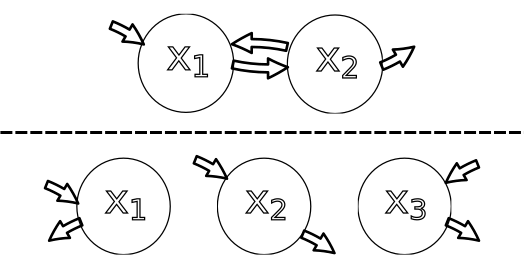
\includegraphics[width=0.5\linewidth]{figs/which_model_more_complex.png}
    \caption{Which model is more complex, the two-compartment model with feedback or the three-compartment model without feedback?
		}
		\label{fig:which_model_more_complex}
\end{figure}

This leads to the problem of how to define complexity for compartmental systems in the first place (Figure~\ref{fig:which_model_more_complex}).
\citet[Chapter 23]{Walter1999} ask a complexity measure/index to have at least the following natural properties:
\begin{enumerate}[(1)]
 \item For a given structure, the index should have its greatest value when the flow rates are even (all the same).
 \item Given two structures with the same number of compartments and even flow rates, the index should have a larger value for the one with more nonzero flow rates.
\end{enumerate}

Many common complexity measures of dynamical systems are closely related to the information content of the system and hence to some kind of entropy.
Two examples are the topological entropy and the Kolmogorov-Sinai/metric entropy.
However, linear autonomous compartmental systems are asymptotically stable.
By Pesin's theorem \citep{Pesin1977UMN}, both the metric- and the topological entropy vanish and cannot serve as a complexity measure here; we need a different concept.

Alternatively, we can interpret compartmental systems as weighted directed graphs.
There are numerous different complexity measures for graphs. 
\citet{Dehmer2011IS} provide a comprehensive overview of the history of graph entropy measures.
Unfortunately, most of such entropy measures are based on the number of vertices, vertex degree, edges, or degree sequence \citep{Trucco1956BoMB}.
Thus, they concentrate on only the structural information of the graph.
\red{The Markov chain maximization in the review paper does the same.}

There are also graph theoretical measures that take edges and weights into account by using probability schemes.
Their drawback is that the underlying meaning of complexity becomes difficult to interpret because the assigned probabilities seem somewhat arbitrary \citep{Bonchev2005}.

Since in the previous chapters we, amongst others, addressed the transit times of particles that travel through the system, we are naturally guided to a different approach.
In terms of a single particle that moves through the system governed by a stochastic process, we can ask how difficult it is for us to guess the particle's current compartment, the particle's next compartment, and the particle's previous compartment.
The more difficult it is to answer these three questions, the higher the complexity of the model should be. 
Consequently, a model's complexity should increase with the number of compartments, the number of fluxes leaving compartments, and the number of fluxes entering compartments.
A weighted average of these numbers seems desirable.
But how to choose the correct weights?

Since in open systems all material that enters the system also exits it later on, in this chapter we try to define a reasonable complexity measure for open compartmental systems based on the Shannon entropy \citep{Shannon1949TUoIP} of the stochastic path covered by a particle from the moment of entering the system until the moment of leaving it.
We further define a model's information content and touch the above mentioned problem of model selection, based on the concept of maximum entropy.


The manuscript is organized as follows.
\red{First we describe compartmental systems in equilibrium, then... and then we compute the three introduced entropy quantities for two carbon cycle models in equilibrium, depending on important parameter values.}

\section{Materials and methods}
First, we introduce some basic notations and well-known properties of Shannon information entropy of random variables and stochastic processes.
Then we present compartmental systems as a means to model material cycle systems that obey the law of mass balance.
Then we consider such systems from a single-particle point of view and define the path of a single particle through the system along with its visited compartments, sojourn times, occupation times, and transit time.
Based on these basic structures of a path, we compute three different types of entropy.
For a better understanding, we provide a summary of the desirable relations among the three different types:
\begin{enumerate}[(1)]
	\item As a particle travels through the system, it jumps a certain number of times to the next compartment until it finally jumps out of the system to the \red{environmental compartment} $d+1$.
	Between two jumps, the particle resides in some compartment.
	Each jump comes with the uncertainties about which compartment will be next and how long will the particle stay there.
	The \emph{entropy rate per jump} measures the average of these uncertainties with respect to the mean number of jumps.
	\item The travel of the particle takes a certain time.
	In each unit time interval before the particle leaves, uncertainties exist whether the particle jumps, where it jumps, and even how often it jumps.
	The mean of these uncertainties over the mean length of the travel interval is measured by the \emph{entropy rate per unit time}.
	\item The \emph{path entropy} measures the entire uncertainty about the particles travel through the system.
	We should be able to compute it if we multiply the mean entropy rate per jump by the mean number of jumps, and also if we multiply the entropy rate per unit time by the mean transit time.
\end{enumerate}


\subsection{Basic ideas of Shannon information entropy}
\label{sec:entropy_basics}

We introduce basic concepts of information entropy along the lines of \citet{Cover2006}.
There are two concepts of entropy of a random variable, depending on whether the random variable has a discrete or a continuous distribution.
Let $Y$ be a discrete real-valued random variable with $d$ distinct values $y_i,\,i=1,2,\ldots, d$ and probability mass function $p$ such that $p(y_i) = p_i\geq 0$ and $\sum_{i=1}^d p_i = 1$ for a probability vector $\vec{p}=(p_i)_{i=1, 2, \ldots,d}$.
Then the \emph{(Shannon information) entropy} of $Y$ and $\vec{p}$ is defined by
\begin{equation*}
  \begin{aligned}
    \H(Y) &= H(\vec{p}) = \H(p_1,p_2,\ldots,p_d)\\
    &= -\suml_{i=1}^d p(y_i)\,\log p(y_i)
    = -\suml_{i=1}^d p_i\,\log p_i
    = -\E\left[\log p(Y)\right],
  \end{aligned}
\end{equation*}
where by convention $0\,\log 0:=0$.
The \emph{(differential) entropy} of a continuous real-valued random variable $Y$ with \pdf\ $f$ is defined by
\begin{equation*}
	\H(Y) = -\int_{-\infty}^{\infty} f(y)\,\log f(y)\dd{y} = -\E\left[\log f(Y)\right].
\end{equation*}
Throughout this manuscript we use Euler's number $e$ as logarithmic base such that the unit of the entropy is nats, if not explicitly stated otherwise.

The entropy $\H(Y)$ of a random variable $Y$ has two intertwined interpretations.
On the one hand, $\H(Y)$ is a measure of uncertainty, \ie, a measure of how difficult it is to predict the outcome of a realization of $Y$.
On the other hand, $\H(Y)$ is also a measure of the information content of $Y$, \ie, a measure of how much information we gain once we learn about the outcome of a realization of $Y$.
It is important to note that, even though their definitions and information theoretical interpretations are quite similar, the Shannon- and the differential entropy have one main difference.
The Shannon entropy is always nonnegative, whereas the differential entropy can have negative values.
Consequently, the Shannon entropy is an absolute measure of information and makes sense in its own right, whereas the differential entropy is not an absolute information measure, is not scale-invariant, and makes sense only in comparison with the differential entropy of another random variable.

Panel A of Fig.~\ref{fig:simple_entropy} depicts the Shannon entropy of a Bernoulli random variable $Y$ with $\P(Y=1)=1-\P(Y=0)=p$ with $p\in[0,1]$.
This random variable could represent the outcome of a coin toss.
We can see that the entropy is low when $p$ is close to $0$ or $1$.
In these cases, we have some information that the coin is biased, and hence we have a preference if we guess the outcome.
The entropy is maximum if the coin is fair ($p=1/2$), since we have no additional information about the outcome of the coin toss.
The Shannon entropy of $Y$ is
\begin{equation*}
	\H(Y) = -p\,\log p - (1-p)\,\log(1-p).
\end{equation*}

Panel B of Fig.~\ref{fig:simple_entropy} shows the differential entropy of an exponentially distributed random variable $Y\sim\Exp(\lambda)$ with rate parameter $\lambda>0$, \pdf\ $f(y) = \lambda\,e^{-\lambda\,y}$ for $y\geq0$, and $\E\left[Y\right]=\lambda^{-1}$.

We can imagine it to represent the duration of stay of a particle in a well-mixed compartment in a linear autonomous compartmental system, where $\lambda$ is the total outflow rate from the compartment.
The higher the outflow rate is, the likelier is an early exit of the particle, and the easier it is to predict the moment of exit.
Hence, the differential entropy decreases with increasing $\lambda$.
It is given by
\begin{equation*}
	\H(Y) = 1-\log\lambda.
\end{equation*}

% \begin{mydef}%[Joint entropy]
% 		Let $Y_1,Y_2$ be two discrete random variables with joint probability mass function $p$ and ranges $R_1$ and $R_2$, respectively.
% 		The \emph{joint entropy} of $Y_1$ and $Y_2$ is defined by
% 		\begin{equation*}
% 			\HJ(Y_1,Y_2) = -\suml_{y_1\in R_1}\suml_{y_2\in R_2} p(y_1,y_2)\,\log p(y_1,y_2) = -\E\left[\log p(Y_1,Y_2)\right].
% 		\end{equation*}
% \end{mydef}
% 
% Note that the joint entropy is symmetric, \ie, $\HJ(Y_1,Y_2) = H(Y_2,Y_1)$.
% 
% \begin{mydef}%[Conditional entropy]
% \label{def:conditional_entropy}
% 	Let $Y_1$ and $Y_2$ be two discrete random variables with joint probability mass function $p$.
% 	Furthermore, let $p_2$ denote the probability mass function of $Y_2$ and denote by $p(y_1\,|\,y_2)$ the conditional probability $\PC(Y_1=y_1\,|\,Y_2=y_2)$.
% 	
% % 	\newpage
% 	Then the \emph{conditional entropy} of $Y_1$ given $Y_2$ is defined by
% 	\begin{equation*}
% 		\begin{aligned}
% 			\HC(Y_1\,|\,Y_2) &= \suml_{y_2\in R_2} \HC(Y_1\,|\,Y_2=y_2)\,p_2(y_2)\\
% 			&= -\suml_{y_2\in R_2} p_2(y_2)\suml_{y_1\in R_1}p(y_1\,|\,y_2)\,\log p(y_1\,|\,y_2)\\
% 			&= -\suml_{y_2\in R_2}\suml_{y_1\in R_1} p(y_1,y_2)\,\log p(y_1\,|\,y_2)\\
% 			&= -\E\left[\log p(Y_1\,|\,Y_2)\right].
% 		\end{aligned}
% 	\end{equation*}
% \end{mydef}
% 
\begin{figure}[htbp]
  \vspace{-0.6cm}
  \centering
  \includegraphics[width=1.0\linewidth]{figs/simple_entropy_py}
  \caption[Entropy of Bernoulli- and exponentially distributed random variables, entropy rate of Poisson process.]{A) Shannon entropy (logarithmic base $2$) of a Bernoulli random variable depending on its success probability $p$.
  B) Differential entropy with logarithmic base $e$ of an exponentially distributed random variable depending on its rate parameter $\lambda$.
  C) Entropy rate of a Poisson process with intensity rate $\lambda$.}
  \label{fig:simple_entropy}
\end{figure}
% 
% The joint entropy of two random variables is the entropy of one variable plus the conditional entropy of the other.
% This is expressed in 
% \begin{equation}\label{eqn:two_expansion_rule}
% 	\HJ(Y_1,Y_2) = \H(Y_2) + \HC(Y_1\,|\,Y_2).
% \end{equation}
% Let $Y_3$ be a third discrete random variable.
% Then
% \begin{equation}\label{eqn:three_expansion_rule}
% 	\HC(Y_1,Y_2\,|\,Y_3) = \HC(Y_1\,|\,Y_3) + \HC(Y_2\,|\,Y_1,Y_3).
% \end{equation}
% 
% Let $Y_1,Y_2,\ldots,Y_n$ be discrete random variables.
% By repeated application of Eq.~\eqref{eqn:two_expansion_rule} and Eq.~\eqref{eqn:three_expansion_rule}, we obtain the \emph{chain rule}
% \begin{equation}\label{eqn:chain_rule}
% 	\HJ(Y_1,Y_2,\ldots,Y_n) = \suml_{k=1}^n \HC(Y_k\,|\,Y_{k-1},\ldots,Y_1).
% \end{equation}
% 
% \begin{myremark}
% 	We defined the joint- and conditional entropy for discrete random variables only.
% 	Analogous definitions can be made for continuous random variables.
% 	Also the chain rule holds for differential entropy.
% \end{myremark}

% \begin{mydef}%[Discrete-time entropy rate]
% \label{def:entropy_rate}
% 	The \emph{entropy rate} of a discrete-time stochastic process $Y=(Y_n)_{n\in \N}$ is defined by
% 	\begin{equation*}
% 		\theta(Y) = \liml_{n\to\infty} \frac{1}{n}\,\HJ(Y_1,Y_2,\ldots,Y_n) = -\frac{1}{n}\,\E\left[\log p_n(Y_1,Y_2,\ldots,Y_n)\right]
% 	\end{equation*}
% 	if the limit exists.
% 	Here, $p_n$ denotes the joint probability mass function of $Y_1,Y_2,\ldots,Y_n$.
% \end{mydef}
% 
% The discrete-time entropy rate describes the long-term average increase of the processes' entropy per time step.
% The statements of the following lemma are proven in \citet[Theorem~4.2.1]{Cover2006}.
% 
% \begin{mylemma}\label{lem:entropy_rate_st_MC}
% 	For a stationary discrete-time stochastic process $Y=(Y_n)_{n\in\N}$, the entropy rate is
% 	\begin{equation*}
% 		\theta(Y) = \liml_{n\to\infty} \HC(Y_n\,|\,Y_{n-1},\ldots,Y_1).
% 	\end{equation*}
% 	Consequently, if $Y$ is a stationary discrete-time Markov chain, its entropy rate is
% 	\begin{equation*}
% 		\theta(Y) = \HC(Y_2\,|\,Y_1).
% 	\end{equation*}
% \end{mylemma}
% 

According to \citet{Dumitrescu1988MICAS} and \citet{Girardin2003JAP} we can extend the concept of entropy to continuous-time stochastic processes $Z=(Z_t)_{\geq0}$.
We first define the entropy of $Z$ on a finite time interval $[0,\,T]$ by
\begin{equation*}
  \H_T(Z) = - \int f_T(z)\,\log f_T(z)\dd{\mu_T(z)},	 
\end{equation*}
where $f_T$ is the \pdf\ of $(Z_t)_{0\leq t\leq T}$ with respect to some reference measure $\mu_T$, if it exists.
Note that by this definition we interpret the entire stochastic process $Z$ on the interval $[0,\,T]$ as a single random variable on the space
\begin{equation*}
  \{z=(z_t)_{t\in[0,\,T]}: z_t\in\R\}.
\end{equation*}
Then the \emph{entropy rate} of $Z$ is defined by
\begin{equation*}
	\theta(Z) = \liml_{T\to\infty} \frac{1}{T}\,\H_T(Z),
\end{equation*}
if the limit exists.

Let $Z\sim\Poi(\lambda)$ be a Poisson process with intensity rate $\lambda>0$ describing the moments of occurrence of certain events.
The interarrival times of $Z$ or the times between events are $\Exp(\lambda)$-distributed, such that in the long run on average the time span between events has length $\lambda^{-1}$.
The entropy of the interarrival times is given by $\H(\Exp(\lambda))=1-\log \lambda)$, and averaging it over the mean interarrival time gives the entropy rate of the Poisson process $Z$ \citep[Section 3.3]{Gaspard1993PR}, \ie,
\begin{equation*}
  \H(Z) = \H(\Poi(\lambda)) = \lambda\,(1-\log \lambda).
\end{equation*}
This entropy rate increases with $\lambda$ with values between $0$ and $1$, where it reaches its maximum, and then it decreases.
This behavior is independent of the unit of $\lambda$, because it is based on the differential entropy of the exponential distribution and hence not scale-invariant.
Consequently, it is no absolute measure of information content, but only useful in comparison to the entropy rate of other stochastic processes.


\subsection{Linear autonomous compartmental systems}\label{sec:one_particle}
Mass-balanced flow of material into a system, within a system and out a a system that consists of several compartments can modeled by so-called compartmental systems \citep{Anderson1983}.
Following \citet{Jacquez1993SIAM}, a \emph{compartment} is an amount of some material that is kinetically homogeneous.
By kinetically homogeneous we mean that the material of a compartment is at all times homogeneous; any material entering the compartment is instantaneously mixed with the material already there.
Hence compartments are always \emph{well-mixed}.
One way to describe compartmental systems is by the $d$-dimensional linear system of ordinary differential equations 
\begin{equation}\label{eqn:lin_CS_sys}
  \deriv{t}\,\vec{x}(t) = \tens{B}\,\vec{x}(t) + \vec{u},\quad t>0,\\
\end{equation}
with some initial condition $\vec{x}(0) = \vec{x}^0\in\R^d$.
The nonnegative vector $\vec{x}(t)$ describes the amount of material in the different compartments at time $t$, the nonnegative vector $\vec{u}$ is the vector of external inputs to the compartments, and the compartmental matrix $\tens{B}\in\R^{d\times d}$ describes the flux rates between the compartments and out of the system.
To ensure that the system is mass balanced, we require the matrix $\tens{B}$ be compartmental, i.e., 
\begin{enumerate}[(i)]
    \item all off-diagonal entries are nonnegative;
    \item all diagonal entries are nonpositive;
    \item all column sums are nonpositive.
\end{enumerate}
The off-diagonal value $B_{ij}$ is the flux rate from compartment $j$ to compartment $i$, the absolute value of the negative diagonal value $B_{jj}$ is the total rate of fluxes out of compartment $j$, and the nonnegative value $z_j=-\sum_{i=1}^d B_{ij}$ is the rate of the flux from compartment $j$ out of the system.
We require additionally that at least one column sum of $\tens{B}$ is strictly negative.
This guarantees that the compartmental system is open in the sense that all material that enters the system will also leave the system at some point in time.
The open compartmental system \eqref{eqn:lin_CS_sys} has a unique steady-state or equilibrium compartment vector $\vec{x}^\ast = -\tens{B}^{-1}\,\vec{u}$ to which $\vec{x}(t)$ converges as $t\to\infty$, independently of the initial vector $\vec{x}^0$.
In this manuscript, we are interested only in systems that have already reached the equilibrium such that $\vec{x}(t)=\vec{x}^\ast$ for all $t>0$.
Note that also nonlinear systems, in which $\tens{B}(\vec{x})$ or $\vec{u}(\vec{x})$ or both can depend on the system content $\vec{x}$, might reach a steady state $\vec{x}^\ast = -[\tens{B}(\vec{x}^\ast)]^{-1}\,\vec{u}(\vec{x}^\ast)$, in which case $\tens{B}=\tens{B}(\vec{x}^\ast)$ and $\vec{u}=\vec{u}(\vec{x}^\ast)$ are constant.
A compartmental system in equilibrium given by Eq. \eqref{eqn:lin_CS_sys} is fully characterized by $\vec{u}$ and $\tens{B}$, and we denote it by $\mathcal{M}=\mathcal{M}(\vec{u},\tens{B})$.


\subsection{The one-particle perspective}
\label{sec:the_one_particle_perspective}
While Eq. \eqref{eqn:lin_CS_sys} describes the movement of bulk material through the system, compartmental systems in equilibrium can also be described probabilistically by considering the random path of a single particle through the system \citep{Metzler2018MGS}.
If $X_t\in\mathcal{S}:=\{1,2,\ldots,d\}$ denotes the compartment in which the single particle is at time $t$, and $X_t=d+1$ if the particle has already left the system, then $X:=(X_t)_{t\geq0}$ is an absorbing continuous-time Markov chain \citep{Norris1997} on $\widetilde{\mathcal{S}}:=\mathcal{S}\cup\{d+1\}$.
Its initial initial distribution is given by $\widetilde{\vec{\beta}}=(\beta_1, \beta_2, \ldots, \beta_d, 0)^T$, where $\vec{\beta}=\vec{u}/\vnorms{\vec{u}}$ and $\beta_j=\P(X_0=j)$ is the probability of the single particle to enter the system through compartment $j$.
The superscript $T$ denotes the transpose of the vector/matrix  and $\vnorms{\vec{u}}=\sum_{i=1}^d |u_i|$ denotes the $l_1$-norm of the vector $\vec{u}$.
The state-transition matrix of $X$ is given by
\begin{equation}\label{eqn:Q}
  \tens{Q} =
  \begin{pmatrix}
    \tens{B} & \vec{0} \\
    \vec{z}^T & 0
  \end{pmatrix},
\end{equation}
and thus
\begin{equation*}
  \P(X_t=i) = (e^{t\,\tens{Q}}\,\vec{\beta})_i = \suml_{j=1}^d (e^{t\,\tens{Q}})_{ij}\,\beta_j, \quad i\in\widetilde{\mathcal{S}},
\end{equation*}
is the probability of the particle to be in compartment $i$ at time $t$ if $i\in\mathcal{S}$ or that the particle has left the system if $i=d+1$.
Here, $e^{t\,\tens{Q}}$ denotes the matrix exponential, and 
\begin{equation*}
  \P(X_t=i\,|\,X_s=j) = (e^{(t-s)\,\tens{Q}})_{ij},\quad s\leq t,\quad i,j\in\widetilde{\mathcal{S}},
\end{equation*}
is the probability that $X$ is in state $i$ at time $t$ given it was in state $j$ at time $s$.
Since the Markov chain $X$ and the compartmental system in equilibrium given by Eq. \eqref{eqn:lin_CS_sys} are equivalent, we can write
\begin{equation*}
  \mathcal{M}=\mathcal{M}(\vec{u},\tens{B}) = \mathcal{M}(X).
\end{equation*}


\subsection{The path of a single particle}
A particle's path through the system from the moment of entering until the moment of exit can be described by
\begin{equation}
  \label{eqn:path}
  \mathcal{P}(X) = ((Y_1=X_0, T_1),(Y_2,T_2),\ldots,(Y_{\mathcal{N}-1},T_{\mathcal{N}-1}), Y_{\mathcal{N}}=d+1),
\end{equation}
where $X$ is the absorbing Markov chain associated to the particle's journey.
The sequence $Y_1,Y_2,\ldots,Y_{\mathcal{N}-1}\in\mathcal{S}$ represents the successively visited compartments along with the associated sojourn times $T_1,T_2,\ldots,T_{\mathcal{N}-1}$, the random variable
\begin{equation*}
  \mathcal{N}:=\inf\,\{n\in\N:\,Y_n=d+1\}
\end{equation*}
denotes the first hitting time of the \emph{embedded jump chain} $Y:=(Y_n)_{n=1,2,\ldots,\mathcal{N}}$ of $X$ \citep{Norris1997}.
With $\lambda_j:=-Q_{jj}$ the one-step transition probabilities of $Y$ are given by, for $i,j\in\widetilde{\mathcal{S}}$,
\begin{equation}\label{eqn:P_ij}
  P_{ij}:=\P(Y_{n+1}=i\,|\,Y_n=j) = 
  \begin{cases}
    0,\quad & i=j\text{ or }\lambda_j=0,\\
    Q_{ij}/\lambda_j,\quad & \text{else}.
  \end{cases}
\end{equation}
We can also write $\tens{P}=\tens{Q}\,\tens{D}^{-1} + \tens{I}$, where
\begin{equation*}
  \tens{D} = \diag\,(\lambda_1,\lambda_2,\ldots,\lambda_d,\lambda_{d+1})
\end{equation*}
is the diagonal matrix with the diagonal entries of $\tens{Q}$ and $\tens{I}$ denotes the identity matrix of appropriate dimension.
Defining the matrix $\tens{P}_{\tens{B}} = (P_{ij})_{i,j\in\mathcal{S}}$, then $\tens{M}:=(\tens{I}-\tens{P}_{\tens{B}})^{-1}$ is the \emph{fundamental matrix} of $Y$, with $\tens{I}\in\R^{d\times d}$ denoting the identity matrix.
The entry $M_{ij}$ denotes the expected numbers of visits to compartment $i$ given that the particle entered the system through compartment $j$.
Consequently, the expected number of visits to compartment $i\in\mathcal{S}$ is given by 
\begin{equation}
  \label{eqn:N_i}
  N_i = (\tens{M}\,\vec{\beta})_i = \left[(\tens{I}-\tens{P}_{\tens{B}})^{-1}\,\vec{\beta}\right]_i 
  = (\tens{D}\,\tens{B}^{-1}\,\vec{\beta})_i
  = \frac{\lambda_i\,x^\ast_i}{\vnorms{\vec{u}}}
\end{equation}
and the total expected number of jumps is given by
\begin{equation*}
  \E\left[\mathcal{N}\right] = \suml_{i=1}^d (\tens{M}\,\vec{\beta})_i+1= \suml_{i=1}^d N_i+1,
\end{equation*}
where we take into account also the first jump into the system.

The last jump, $\mathcal{N}$, leads the particle out of the system such that at the moment of this last jump $X$ takes on the value $d+1$.
This last jump happens at the absorption time of the Markov chain $X$, which is defined as
\begin{equation*}
   \TT := \inf\,\{t>0: X_t=d+1\}.
\end{equation*}
The absorption time is phase-type distributed \citep{Neuts1981}, $\TT\sim\PH(\vec{\beta},\tens{B})$, with \pdf
\begin{equation*}
  f_{\TT}(t) = \vec{z}^T\,e^{t\,\tens{B}}\,\vec{\beta},\quad t\geq0.
\end{equation*}
It can be shown \citep[Section 3.2]{Metzler2018MGS} that the mean or expected value of $\TT$ equals the resident time \citep{Sierra2016GlobChangBiol} of system \eqref{eqn:lin_CS_sys} in equilibrium and is given by total stocks over total fluxes, i.e., 
\begin{equation*}
  \E\left[\TT\right] = \frac{\vnorms{\vec{x}^\ast}}{\vnorms{\vec{u}}}.
\end{equation*}
Furthermore, it is obvious by construction that $\sum_{k=1}^{\mathcal{N}-1} T_k = \TT$.
If we denote by $\mathbbm{1}_{\{A\}}$ the indicator function of the logical expression $A$, given by
\begin{equation*}
  \mathbbm{1}_{\{A\}} =
  \begin{cases}
    1, \quad A\text{ is true},\\
    0, \quad\text{else},
  \end{cases}
\end{equation*}
then $\sum_{k=1}^{\mathcal{N}-1} \mathbbm{1}_{Y_k=j}\,T_k$ is the time that the particle spends in compartment $j$.
This time is called \emph{occupation time} of $j$ and its mean is given by \citep[Section 3.3]{Metzler2018MGS}
\begin{equation}
  \label{eqn:occupation_time}
  \E\left[O_j\right] = \frac{x^\ast_j}{\vnorms{\vec{u}}},
\end{equation}
which induces $\E\left[\TT\right] = \sum_{j=1}^d \E\left[O_j\right]$.


% We come back to the $d$-dimensional open linear autonomous system~\eqref{eqn:CS_ODE_la2} in equilibrium from Chapter~\ref{chapter:in_equilibrium} and denote it by $M$.
% Let $X$ denote the associated absorbing continuous-time Markov chain and $Z$ the infinite continuous-time process from Eq.~\eqref{eqn:Z}.
% The system is given by
% \begin{equation}\label{eqn:CS_ODE_la2_eq_chapter}
% 	\begin{aligned}
% 		\deriv{t}\,\vec{x}(t) &= \tens{B}\,\vec{x}(t)+\vec{u},\quad t>0,\\
% 		\vec{x}(0) &= \vec{x}^\ast.
% 	\end{aligned}
% \end{equation}
% This system might have been linear from the beginning or it might result from an autonomous nonlinear system that has reached an equilibrium.
% Since $\tens{B}$ is invertible, by Proposition~\ref{proposition:LA_exp_stable} this system has a globally attracting fixed point $\vec{x}^\ast=-\tens{B}^{-1}\,\vec{u}$, so it has no positive Lyapunov exponents.
% Consequently, its metric- and topological entropy are zero by Pesin's theorem and cannot serve as complexity measures.
% We need a different approach to define a complexity measure for such systems.
% 
% To that end, we look at the path that a single particle covers while it travels through the system.
% This path is a finite sequence of pairs $(\zeta_n,T_n)$, where $\zeta_n$ stands for the $n$th compartment visited by the particle and $T_n$ for the sojourn time in the $n$th compartment.
% A particle leaving the system is modeled as entering the so-called \emph{environmental compartment} $d+1$.
% The particle is then supposed to stay there for an infinitesimal amount of time before it reenters the system.
% The particle's then infinite path $\mathcal{P}_\infty:=((\zeta_n,T_n))_{n\in\N}$ consists of two Markov processes. 
% The first one, $\zeta=(\zeta_n)_{n\in\N}$ with values in 
% \begin{equation*}
% 	\widetilde{S}=\{1,2,\ldots,d,d+1\}
% \end{equation*}	
% describes the sequence of visited compartments and is a discrete-time Markov chain.
% The second one, the sojourn-time process $(T_n)_{n\in\N}$, with values in $\mathbb{R}_{+}$ describes the sequence of sojourn times. 
% % The compartment chain $\zeta$ is independent of the sojourn-time process, but the sojourn-time process depends on $\zeta$, because the current compartment determines the current sojourn-time distribution.
% If at time step $n\in\N$ the particle is in compartment $j\in S=\{1,2,\ldots,d\}$, then $T_n\sim\operatorname{Exp}(\lambda_j)$, where $\lambda_j:=-B_{jj}$.
% Since we cannot model an infinitesimal sojourn time for the environmental compartment $d+1$, we define its sojourn-time distribution to be $\operatorname{Exp}(\lambda_{d+1})$ for $\lambda_{d+1}:=1$ and correct for it later.



\subsection{Path entropy, entropy rate per unit time, entropy rate per jump}
\label{sec:path_entropy}
The path $\mathcal{P}$ given by Eq. \eqref{eqn:path} can be interpreted in three different ways.
Each of these ways leads to a different interpretation of the path's entropy.
First, we can look at $\mathcal{P}$ as the result of bookkeeping of the absorbing continuous-time Markov chain $X$, where as a sequence of pairs on the occasion of a jump we note down the old compartment of the traveling particle and the associated time the particle spent in this compartment.
Second, we can consider the path as a discrete-time process.
In each time step $n$, we choose randomly a new compartment $Y_{n+1}$ and an associated sojourn time $T_{n+1}$ of the particle in this compartment.
Third, we can look at $\mathcal{P}$ as a single random variable with values in the space of all possible paths.
Based on the latter interpretation we now derive the path entropy.

We are interested in the uncertainty/information content of the path $\mathcal{P}(X)$ of a single particle.
Along the lines of \citet{Albert1962AMS}, we construct a space $\wp$ that contains all possible paths that can be taken by a particle that runs through the system until it leaves.
Let $\wp_n:=(S\times\R_+)^n\times\{d+1\}$ denote the space of paths that visit $n$ compartments/states before ending up in the environmental compartment/absorbing state $d+1$.
By $\wp:=\bigcup_{n=1}^{\infty}\wp_n$ denote the space of all eventually absorbed paths.
Note that, since $\tens{B}$ is invertible, a path through the system is finite with probability $1$.
Let $l$ denote the Lebesgue measure on $\R_+$ and $c$ the counting measure on $S$.
Furthermore, let $\sigma_n$ be the sigma-finite product measure on $\wp_n$.
It is defined by $\sigma_n:=(c\otimes l)^n \otimes c$.
Almost all sample functions of $(X_t)_{t\geq0}$ can be represented as a point $p\in\wp$ \citep[Chapter~VI]{Doob1953}.
Consequently, we can represent $X$ by a finite-length path $\mathcal{P}(X)=((Y_1,T_1),(Y,T_2),\ldots,(Y_n,T_n),Y_{n+1})$ for some $n\in\N$, where $Y_{n+1}=d+1$.

For each set $W\subseteq\wp$ for which $W\cap \wp_n$ is $\sigma_n$-measurable for each $n\in\N$, we define $\sigma^\ast(W) := \sum_{n=1}^{\infty} \sigma_n(W\cap\wp_n)$.
It is defined on the $\sigma$-field $\mathcal{F}^\ast$ which is the smallest $\sigma$-field containing all sets $W\subseteq\wp$ whose projection on $\R^n_+$ is a Borel set for each $n\in\N$.
Let $\sigma$ be a measure on \emph{all} sample functions, defined for all subsets $W$ whose intersection with $\wp$ is in $\mathcal{F}^\ast$. 
We define it by $\sigma(W):=\sigma^*(W\cap\wp)$.

Let $p=((x_1,t_1),(x_2,t_2,),\ldots,(x_n,t_n),d+1)\in\wp$ for some $n\in\N$.
For $i\neq j$, we denote by $N_{ij}(p)$ the total number of path $p$'s transitions from $j$ to $i$ and by $R_j(p)$ the total amount of time spent in $j$.

\begin{lemma}\label{lem:path_pdf}
	The \pdf\ of $\mathcal{P}=\mathcal{P}(X)$ with respect to $\sigma$ is given by
	\begin{align*}
		f_{\mathcal{P}}(p) = \beta_{x_1}\Bigg(\prodl_{j=1}^d\,\prodl_{i=1,i\neq j}^{d+1} &(Q_{ij})^{N_{ij}(p)}\Bigg)\prodl_{j=1}^d e^{-\lambda_j\,R_j(p)},\\
		& p=((x_1,t_1),(x_2,t_2),\ldots,(x_n,t_n),d+1)\in\wp.
	\end{align*}
\end{lemma}

\begin{proof}
	Let $x_1,x_2,\ldots,x_n\in S$, $x_{n+1}=d+1$, and $t_1,t_2,\ldots,t_n\in\R_p$.
	Since
	\begin{align*}
		&\P((Y_1=x_1,T_1\leq t_1),\ldots,\,(Y_n=x_n,T_n\leq t_n),\, Y_{n+1}=d+1) \\
		&\qquad= \P(Y_{n+1}=d+1\,|\,Y_n=x_n)\,\prodl_{k=1}^n \P(Y_k=x_k,T_k\leq t_k\,|\,Y_{k-1}=x_{k-1})\\
		&\qquad= P_{d+1,x_n}\left[\prodl_{k=2}^n P_{x_{k} x_{k-1}}\left(1-e^{-\lambda_{x_k}\,t_k}\right)\right] \beta_{x_1}\left(1-e^{-\lambda_{x_1}\,t_1}\right)\\
		&\qquad= \intl_{\mathbb{T}_n} \beta_{x_1}\prodl_{k=1}^n Q_{x_{k+1}x_k}\,e^{-\lambda_{x_k}\,\tau_k}\,\mathrm{d}\tau_1\mathrm{d}\tau_2\cdots\mathrm{d}\tau_n
	\end{align*}
	with $\mathbb{T}_n=\{(\tau_1,\tau_2,\ldots,\tau_n)\in\R^n_+:\,0\leq\tau_1\leq t_1,0\leq\tau_2\leq t_2,\ldots,0\leq\tau_n\leq t_n\}$,
	the \pdf\ of $\mathcal{P}=\mathcal{P}(x)$ with respect to $\sigma$ is given by
	\begin{align*}
		f_{\mathcal{P}}(p) = \beta_{x_1}\prodl_{k=1}^n &Q_{x_{k+1}x_k}\,e^{-\lambda_{x_k}\,t_k},\\
		& p=((x_1,t_1),(x_2,t_2),\ldots,(x_n,t_n),d+1)\in\wp.
	\end{align*}
	The term $Q_{x_{k+1}x_k}=Q_{ij}$ enters exactly $N_{ij}(p)$ times.
	Furthermore,
	\begin{align*}
		\prodl_{k=1}^n e^{-\lambda_{x_k}\,t_k} &= \prodl_{k=1}^n\,\prodl_{j=1}^d \mathbbm{1}_{\{x_k=j\}}\,e^{-\lambda_j\,t_k}
		= \prodl_{j=1}^d e^{-\lambda_j\,\suml_{k=1}^n \mathbbm{1}_{\{x_k=j\}}\,t_k}
		= \prodl_{j=1}^d e^{-\lambda_j\,R_j(p)}.
	\end{align*}
	We make the according substitutions and the proof is finished.
\end{proof}

The \emph{entropy of the absorbing continuous-time Markov chain} $X$ is equal to the entropy on the random but finite time horizon $[0,\,\TT]$, which in turn equals the entropy of a single particle's path $\mathcal{P}$ through the system.

\begin{theorem}\label{thm:entropy_of_X}
	The entropy of the absorbing continuous-time Markov chain $X$ is given by
	\begin{equation}
    \label{eqn:H_X}
    \begin{aligned}
      \H(X) &= \H(\mathcal{P})\\
      &= -\suml_{i=1}^d\beta_i\,\log\beta_i\\
      &\quad + \suml_{j=1}^d \frac{x^\ast_j}{\vnorms{\vec{u}}}\left[\suml_{i=1,i\neq j}^d \,B_{ij}\,(1-\log B_{ij}) + z_j\,(1-\log z_j)\right].
    \end{aligned}
	\end{equation}
\end{theorem}

\begin{proof}
	Let $X$ have the finite path representation 
	\begin{equation*}
		\mathcal{P}=\mathcal{P}(X)=((Y_1,T_1),(Y_2,T_2),\ldots,(Y_n,T_n),d+1)
	\end{equation*}
	for some $n\in\N$, and denote by $f_{\mathcal{P}}$ its \pdf.
	Then, by Lemma~\ref{lem:path_pdf},
	\begin{equation*}
		-\log f_{\mathcal{P}}(\mathcal{P}) = -\log\beta_{Y_1} - \suml_{j=1}^d\,\suml_{i=1,i\neq j}^{d+1}N_{ij}(\mathcal{P})\,\log Q_{ij} + \suml_{j=1}^d \lambda_j\,R_j(\mathcal{P}).
	\end{equation*}
	We compute the expectation and get
	\begin{align*}
		\H(X) &= \H(\mathcal{P}) = -\E\left[\log f_{\mathcal{P}}(\mathcal{P})\right]\\
		&= -\E\left[\log\beta_{Y_1}\right] - \suml_{j=1}^d\,\suml_{i=1,i\neq j}^{d+1}\E\left[N_{ij}(\mathcal{P})\right]\,\log Q_{ij} + \suml_{j=1}^d \lambda_j\,\E\left[R_j(\mathcal{P})\right]\\
		&= \H(Y_1) + \suml_{j=1}^d \lambda_j\,\E\left[R_j(\mathcal{P})\right] - \suml_{j=1}^d\,\suml_{i=1,i\neq j}^{d+1}\E\left[N_{ij}(\mathcal{P})\right]\,\log Q_{ij}.
	\end{align*}
	Obviously, $\E\left[R_j(\mathcal{P})\right]=\E\left[O_j\right]=x^\ast_j/\vnorms{\vec{u}}$ is the mean occupation time of compartment $j\in S$ by $X$.
	Furthermore, for $i\in\widetilde{S}$ and $j\in S$ such that $i\neq j$, by Eqs.~\eqref{eqn:N_i} and~\eqref{eqn:P_ij},
	\begin{equation*}
		\E\left[N_{ij}(\mathcal{P})\right] = \E\left[N_j(\mathcal{P})\right]\,P_{ij} = 
		\begin{cases}
			\frac{x^\ast_j}{\vnorms{\vec{u}}}\,B_{ij},\quad & i\leq d,\\
			\frac{x^\ast_j}{\vnorms{\vec{u}}}\,z_j,&i=d+1.
		\end{cases}
	\end{equation*}
	Together with $\lambda_j=\sum_{i=1,i\neq j}^{d} B_{ij}+z_j$, we obtain
	\begin{align*}
		\H(X) &= \H(Y_1) + \suml_{j=1}^d \frac{x^\ast_j}{\vnorms{\vec{u}}}\left[\left(\suml_{i=1,i\neq j}^d B_{ij}+z_j\right) - \suml_{i=1,i\neq j}^d B_{ij}\,\log B_{ij} - z_j\,\log z_j\right]\\
		&= -\suml_{i=1}^d \beta_i\log\beta_i + \suml_{j=1}^d \frac{x^\ast_j}{\vnorms{\vec{u}}} \left[\suml_{i=1,i\neq j}^d B_{ij}\,(1-\log B_{ij}) + z_j\,(1-\log z_j)\right].
	\end{align*}
\end{proof}

By some simple substitutions and rearrangements, we obtain two representations of $\H(X)=\H(\mathcal{P})$ that are easy to interpret.

\begin{proposition}\label{prop:entropy_of_X}
	We
	The entropy of the absorbing continuous-time Markov chain $X$ is also given by
	\begin{equation}
	  \label{eqn:H_occupation_time}
	  \H(X) = \H(\vec{\beta}) + \suml_{j=1}^d \E\left[O_j\right] \left(\suml_{i=1,\,i\neq j}^d \theta(\Poi(B_{ij})) + \theta(\Poi(z_j))\right)
	\end{equation}
	and
	\begin{equation}
	  \label{eqn:H_number_of_visits}
	  \begin{aligned}
      \H(X)& = \H(\vec{\beta})\\
      &\quad + \suml_{j=1}^d \E\left[N_j\right]\, \bigg(\H(\Exp(\lambda_j)) + \H(P_{1,j}, P_{2, j},\ldots,P_{d, j}, P_{d+1,j})\bigg).
    \end{aligned}
  \end{equation}
\end{proposition}

\begin{proof}
  By virtue of Eq. \eqref{eqn:H_occupation_time} we replace $x^\ast_j/\vnorms{\vec{u}}$ by $\E\left[O_j\right]$ in Eq. \eqref{eqn:H_X} and take into account that the entropy rate of a Poisson process with intensity rate $\lambda$ equals $\lambda\,(1-\log \lambda)$ to prove Eq. \eqref{eqn:H_occupation_time}.
  To prove Eq. \eqref{eqn:H_number_of_visits} we use Eq. \eqref{eqn:N_i} to replace $x^\ast_j/\vnorms{\vec{u}}$ in Eq. \eqref{eqn:H_X} by $\E\left[N_j\right]/\lambda_j$ and obtain
  \begin{equation*}
    \begin{aligned}
      \H(X) &= -\suml_{i=1}^d\beta_i\,\log\beta_i\\
      &\quad + \suml_{j=1}^d \E\left[N_j\right]\left((1-\log \lambda_j) - \suml_{i=1,i\neq j}^d \frac{B_{ij}}{\lambda_j}\,\log \frac{B_{ij}}{\lambda_j} - \frac{z_j}{\lambda_j}\,\log \frac{z_j}{\lambda_j}\right).
    \end{aligned}
	\end{equation*}
	Here, $(1-\log \lambda_j)$ is the entropy of an exponential random variable with rate parameter $\lambda_j$.
	Using the definition \eqref{eqn:P_ij} of $P_{ij}$ we replace $B_{ij}/\lambda_j$ for $i\in\mathcal{S}$ and $z_j/\lambda_j$ by $P_{d+1,j}$ ad finish the proof.
\end{proof}

We now define the \emph{path entropy of the compartmental system in equilibrium} $\mathcal{M}$, given by Eq. \eqref{eqn:lin_CS_sys}, as the path entropy of its associated continuous-time Markov chain $X$, i.e.
\begin{equation*}
  \H(\mathcal{M}):=\H(X)=\H(\mathcal{P}).
\end{equation*}

For a one-dimensional compartmental system $\mathcal{M}_\lambda$ in equilibrium with rate $\lambda>0$ and positive external input given by
\begin{equation}
  \deriv{t}\,x(t) = -\lambda\,x(t) + u,\quad t>0,
\end{equation}
the entropy of the initial distribution vanishes, and we obtain
\begin{equation*}
  \H(\mathcal{M}_\lambda) = \frac{x^\ast}{u}\,\lambda\,(1-\log\,\lambda) = \frac{1}{\lambda}\,\lambda\,(1-\log\,\lambda) = 1-\log\,\lambda,
\end{equation*}  
which which equals the differential entropy $1-\log\lambda$ of the exponentially distributed mean transit time $\TT_\lambda\sim\Exp(\lambda)$, reflecting that the only uncertainty of the particle's path in a one-pool system is the time of the particle's exit.
The exponential distribution with rate parameter $\lambda$ is the distribution of the interarrival time of a Poisson process wit intensity rate $\lambda$.
Hence, we can interpret $\H(\mathcal{M}_\lambda) = \lambda^{-1}\,\lambda\,(1-\lambda)$ as the instantaneous Poisson entropy $\lambda\,(1-\lambda)$ multiplied with the expected duration $\E\left[\TT\right]=\lambda^{-1}$ of the particle's stay in the system.

Migrating to a $d$-dimensional system, we can interpret $\H(\mathcal{M})$ as the entropy of a continuous-time process in the light of Eq. \eqref{eqn:H_occupation_time} and as the entropy of a discrete-time process in the light of Eq. \eqref{eqn:H_number_of_visits}.
In both interpretation represents the first term $\H(\vec{\beta})=\H(X_0)=\H(Y_1)$ the uncertainty of the first pool through which the particle enters the system.
In the continuous-time interpretation, the uncertainty of the subsequent travel is the weighted average of the overlapping Poisson processes describing the instantaneous uncertainty of possible jumps of the particle inside the system ($\theta(\Poi(B_{ij}))$) and out of the system ($\theta(\Poi(z_j))$), where the weights are the expected occupation times of the different compartments. 
In the discrete-time interpretation, the subsequent travel's uncertainty is the average of uncertainties associated to each pool, weighted by the number of visits to the respective pools.
The uncertainties associated to each pool comprises the uncertainty of the length of the stay in the pool ($\H(\Exp(\lambda_j))$) and the uncertainty of where to jump afterwards ($\H(P_{1,j},\ldots,P_{d+1,j})$).

% The path entropy of a compartmental system depends heavily on the system's speed or the average path length $\E\left[\TT\right]$, which can easily be seen from $\mathcal{M}_\lambda=1-\,\log\,\lambda$ for a one-pool system.
% The smaller $\lambda$, the slower the system and the higher the uncertainty of the particles exit from the system, hence the higher the path entropy.
% 
% In summary, the path entropy is the uncertainty of the traveling particle's first pool, all its possible transition to other pools, and its time of exit from the system.
% A slow serial system with no jump uncertainty can have higher or lower uncertainty than a fast system with high jump uncertainties \red{example, part of discussion?}

The two interpretations of the path entropy $\H(\mathcal{M})$ (as a time-continuous or time-discrete process) motivate two different entropy rates.
The \emph{entropy rate per unit time} is defined as
\begin{equation*}
  \theta(\mathcal{M}) = \frac{\H(\mathcal{M})}{\E\left[\TT\right]}
\end{equation*}
and the \emph{entropy rate per jump} as
\begin{equation*}
  \theta_J(\mathcal{M}) = \frac{\H(\mathcal{M})}{\E\left[\mathcal{N}\right]}.
\end{equation*}

% \begin{myprop}
% 	The entropy $\H(X)$ is consistent with the entropy rate per jump $\theta(\Pinfty)$ and the entropy rate per unit time $\theta(Z)$.
% 	More precisely,
% 	\begin{equation*}
% 		\H(X) = (1+\MFHT)\,\theta(\Pinfty) = \E\left[\TT\right]\,\theta(Z).
% 	\end{equation*}
% \end{myprop}
% 
% \begin{proof}
% 	The relation $\H(X) = \E\left[\TT\right]\,\theta(Z)$ is immediately obvious from Proposition~\ref{prop:theta_Z}.
% 	From Proposition~\ref{prop:entropy_rate_jump} and Lemma~\ref{lem:entropy_rate_compartment_chain}, we have
% 	\begin{align*}
% 		\theta(\Pinfty) &= \suml_{j=1}^d\pi_j\,(1-\log\lambda_j) + 
% 		\suml_{j=1}^d \pi_j \left[\suml_{i=1,i\neq j}^d -\frac{B_{ij}}{\lambda_j}\,\log\left(\frac{B_{ij}}{\lambda_j}\right) - \frac{z_j}{\lambda_j}\,\log\left(\frac{z_j}{\lambda_j}\right)\right]\\
% 		&\qquad -\pi_{d+1}\,\suml_{i=1}^d \beta_i\,\log\beta_i
% 	\end{align*}
% 	With Eqs.~\eqref{eqn:pi_d} and~\eqref{eqn:pi_dp1}, we obtain
% 	\begin{align*}
% 		(1+\MFHT)\,\theta(\Pinfty) &= \suml_{j=1}^d\frac{x^\ast_j}{\vnorms{\vec{u}}}\,\lambda_j\,(1-\log\lambda_j)\\
% 		&\qquad + \suml_{j=1}^d\frac{x^\ast_j}{\vnorms{\vec{u}}} \left[\suml_{i=1,i\neq j}^d -B_{ij}\,\log\left(\frac{B_{ij}}{\lambda_j}\right) - z_j\,\log\left(\frac{z_j}{\lambda_j}\right)\right]\\
% 		&\qquad -\suml_{i=1}^d \beta_i\,\log\beta_i\\
% 		&= \suml_{j=1}^d\frac{x^\ast_j}{\vnorms{\vec{u}}}\,\left(\suml_{i=1,i\neq j}^d B_{ij}+z_j\right)\,(1-\log\lambda_j)\\
% 		& \qquad +\suml_{j=1}^d\frac{x^\ast_j}{\vnorms{\vec{u}}} \left[\suml_{i=1,i\neq j}^d B_{ij}(\,\log\lambda_j-\log B_{ij}) + z_j\,(\log\lambda_j-\log z_j)\right]\\
% 		&\qquad -\suml_{i=1}^d \beta_i\,\log\beta_i\\
% 		&= -\suml_{i=1}^d\beta_i\,\log\beta_i + \suml_{j=1}^d\frac{x^\ast_j}{\vnorms{\vec{u}}} \left[\suml_{i=1,i\neq j}^d B_{ij}\,(1-\log B_{ij}) + z_j\,(1-\log z_j)\right]\\
% 		&= \H(X).
% 	\end{align*}
% \end{proof}
% 
% \begin{myremark}
% 	Analogously to the interpretation of $\theta(Z)$ in Remark~\ref{rem:Poisson_interpretation}, we can interpret the entropy of $X$ as
% 	\begin{equation*}
% 		\H(X) = \H(\text{entry}) + \suml_{j=1}^d \E\left[O_j\right] \left[\suml_{i=1,i\neq j}^d \H(\text{Poisson(}i\,|\,j\text{)})+\H(\text{Poisson(exit}\,|\,j))\right].
% 	\end{equation*}	
% \end{myremark}
% 
% \begin{mydef}
% 	If $\vec{u}\in\Rpd$, and $\tens{B}\in\R^{d\times d}$ is compartmental and invertible, then we denote by $(\vec{u},\tens{B})$ the linear autonomous compartmental system~\eqref{eqn:CS_ODE_la2_eq_chapter} and by $X$, $\Pinfty$, and $Z$ the associated absorbing continuous-time Markov chain, infinite path, and infinite continuous-time path, respectively.
% 	
% 	Furthermore, the \emph{path entropy} of $M=(\vec{u},\tens{B})$ is defined as $\HP(M):=\H(X)$, its \emph{entropy rate per jump} by $\thetaPinfty(M):=\theta(\Pinfty)$, and its \emph{entropy rate per unit time} by $\thetaZ(M):=\theta(Z)$.
% \end{mydef}

\subsection{Maximum entropy principle}

\subsection{Structural model identification}


\section{Results/Examples}

\subsection{Simple examples}
From Table~\ref{fig:entropy_table} we can see that depending on the connections between compartments smaller systems can have path entropy and entropy rates than bigger systems, even systems with more compartments can theoretically have higher entropy.
Furthermore, we see that the system with the highest path entropy does neither have the highest entropy rate per unit time nor per jump.
Adding connections to a system, one would expect higher path entropy, but the path entropy might increase because the new connection potentially provides a faster way out out the system.

\begin{table}[htbp]
  \centering
  
\includegraphics[width=1.0\linewidth]{figs/entropy_table}
  \caption[Overview of different entropies of simple models with different structures.]{Overview of different entropies     of simple models with different structures.
  The columns from left to right represent a schematic of the model, its mathematical representation, its entropy rate per jump, its entropy rate per unit time, its mean transit time, and its path entropy.
  Underlined numbers are the highest values per column.
  \red{The two gray rows emphasize the examples of the model structures considered at the beginning of the chapter in Fig.~\ref{fig:which_model_more_complex}.}
  \red{include also mean number of jumps, to save space use $\dot{x}$, introduce in text}
  }
  \label{fig:entropy_table}
\end{table}


\subsection{A linear autonomous global carbon cycle model}
\label{subsec:example_1}
We consider the global carbon cycle model introduced by \citet{Emanuel1981} (Fig.~\ref{fig:Emanuel_model}).
\begin{SCfigure}%[htbp]
    \centering
    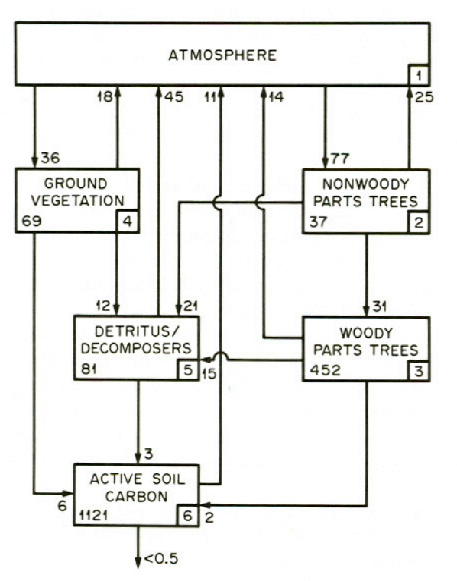
\includegraphics[width=0.5\linewidth]{figs/Emanuel_model}
    \caption[Schematic of the linear autonomous global carbon cycle model in steady state introduced by \citet{Emanuel1981}.]{Schematic of the linear autonomous global carbon cycle model in steady state introduced by \citet{Emanuel1981}. 
      The model comprises five compartments: non-woody tree parts $x_1$ (2; $37\,\peta\gC$), woody tree parts $x_2$ (3; $452\,\peta\gC$), ground vegetation $x_3$ (4; $69\,\peta\gC$), detritus/decomposers $x_4$ (5; $81\,\peta\gC$), and active soil carbon $x_5$ (6; $1,121\,\peta\gC$). The atmosphere (1) is considered to be outside of the modeled system but provides the system with external inputs and receives external outputs from it. Numbers next to arrows indicate fluxes between compartments in $\peta\gC\,\yr^{-1}$. (Figure extracted from \citealt{Emanuel1981})}\label{fig:Emanuel_model}
\end{SCfigure}
The model comprises five compartments: non-woody tree parts $x_1$, woody tree parts $x_2$, ground vegetation $x_3$, detritus/decomposers $x_4$, and active soil carbon $x_5$.
We introduce an environmental rate modifier $\xi$ which controls the speed of the system.
This parameter could potentially increase and speed up the system with increasing global Earth surface temperature.
Since the model is considered to be in equilibrium, the initial state is negligible and, the model is given by
\begin{equation*}
    \deriv{t}\vec{x}(t) = \tens{B}\,\vec{x}(t) + \vec{u},\quad t>0,
\end{equation*}
where the input vector is given by 
\begin{equation*}
  \vec{u} = (77.00;\,0.00;\,36.00;\,0.00;\,0.00)^{\transpose}\, \peta\gC\,\yr^{-1}
\end{equation*}
and the compartmental matrix by
\begin{equation*}
    \tens{B} = \left(\begin{matrix}
      -77/37 &       0 &      0 &      0 & 	  0\\
       31/37 & -31/452 &      0 &      0 & 	  0\\
	   0 &       0 & -36/69 &      0 & 	  0\\
       21/37 &  15/452 &  12/69 & -48/81 & 	  0\\
	   0 &   2/452 &   6/69 &   3/81 & -11/1121
	 \end{matrix}\right)\,\yr^{-1},
\end{equation*}
where the numbers are chosen as in \citet{Thompson1999GCB}. 
The input vector is expressed in units of petagrams of carbon per year ($\peta\gC\,\yr^{-1}$) and the fractional transfer coefficients in units of per year ($\yr^{-1}$).
Because $\tens{B}$ is a lower triangular matrix, the model contains no feedbacks.
For every value of $\xi$ the system has a different steady state (Fig.\ref{fig:Emanuel_entropies}, panel A).
The higher the value of $\xi$, the faster is the system, which makes the mean transit time (panel B) decrease and because of shorter paths also the path entropy (panel D) decreases.
Since $\xi$ has no impact on the structure of the model, the mean number of jumps (panel C) remains unaffected.
Nevertheless, the entropy rate per jump (panel F) decreases with increasing $\xi$ because the path entropy of the system decreases.
The entropy rate per unit time increases until $\xi\approx6$, while the mean transit time decreases faster than the path entropy, and then trend turns around and the entropy rate per unit time decreases (panel E).
Orange lines in panel D and E show the respective entropy values for a one-pool system with the same mean transit time.
The blue and orange lines intersect at $\xi\approx4.31$.

\begin{figure}[htbp]
    \centering
    \includegraphics[width=1.0\linewidth]{figs/Emanuel_entropies}
    \caption[Entropy related quantities of the model introduced by \citet{Emanuel1981}.]{
    A) Equilibrium carbon stocks. B)--F) Entropy related quantities of the global carbon cycle model introduced by \citet{Emanuel1981} in dependence on the environmental rate coefficient $\xi$ (blue lines).
    Orange lines correspond to the quantities derived from a one-pool model with the same speed.
    Vertical gray lines show $\xi=1$, the original speed of the model.}
    \label{fig:Emanuel_entropies}
\end{figure}

\subsection{A nonlinear autonomous soil organic matter decomposition model}
\label{subsec:example_2}
Consider the nonlinear autonomous compartmental system
\begin{equation}\label{eqn:nonlinear_inh}
  \deriv{t} \vec{x}(t) = \tens{B}(\vec{x}(t))\,\vec{x}(t) + \vec{u}, \quad t>0,
\end{equation}
where $\tens{B}:\R^d\to \R^{d\times d}$ is a matrix-valued mapping.
In this setup, the fractional transfer coefficients are not constant but depend on the system's content.

Assume now that system~\eqref{eqn:nonlinear_inh} is in a steady state $\vec{x}^\ast$.
From $\mathrm{d}\,\vec{x}^\ast/\mathrm{d}\,t = 0$ follows that the compartment contents $x^\ast_j$ do not change in time, and the mapping $\tens{B}$ turns into a matrix with constant coefficients. 
Hence, if we assume the nonlinear autonomous compartmental system~\eqref{eqn:nonlinear_inh} to be in a steady state, we can treat it as a linear autonomous compartmental system.

As an example, consider the nonlinear two-compartment carbon cycle model described by \citet{Wang2014BG} (Fig.~\ref{fig:Wang_model}).
\begin{figure}[htbp]
    \centering
    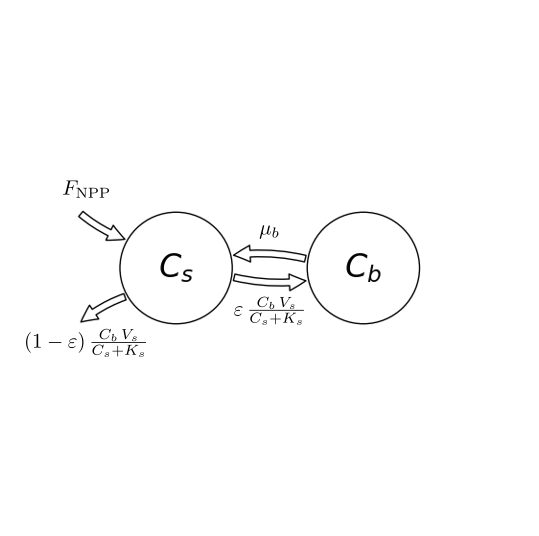
\includegraphics[width=0.5\linewidth]{figs/Wang_model.png}
    \caption[Schematic of the nonlinear autonomous carbon cycle model introduced by \citet{Wang2014BG}.]{Scheme of the nonlinear autonomous carbon cycle model introduced by \citet{Wang2014BG}. 
    The two compartments $C_s$ and $C_b$ are here denoted by SOC (substrate organic carbon) and MIC (microbial biomass carbon), the external input flux $F_{\NPP}$ is denoted by \emph{Inputs}, the maximum rate of soil carbon assimilation by $V_s$, the half saturation constant by $K_s$, the carbon use efficiency by $\varepsilon$, and the turnover rate of microbial biomass by $\mu_b$, respectively.
      (Figure extracted from \citet{Wang2014BG})}\label{fig:Wang_model}
\end{figure}
We denote by $C_s$ and $C_b$ soil organic carbon and soil microbial biomass ($\gC\,\meter^{-2}$), respectively, by $\varepsilon$ the carbon use efficiency or fraction of assimilated carbon that is converted into microbial biomass (unit-less), by $\mu_b$ the turnover rate of microbial biomass per year ($\yr^{-1}$), by $F_{\NPP}$ the carbon influx into soil ($\gC\,\meter^{-2}\,\yr^{-1}$), and by $V_s$ and $K_s$ the maximum rate of soil carbon assimilation per unit microbial biomass per year ($\yr^{-1}$) and the half-saturation constant for soil carbon assimilation by microbial biomass ($\gC\,\meter^{-2}$), respectively.
Then, we can describe the model by
\begin{equation*}
    \deriv{t}\,\left(\begin{matrix}C_{s}\\C_{b}\end{matrix}\right) = \left(\begin{matrix}- \lambda(\vec{x}) & \mu_{b}\\\varepsilon \lambda(\vec{x}) & - \mu_{b}\end{matrix}\right) \, \left(\begin{matrix}C_{s}\\C_{b}\end{matrix}\right) + \left(\begin{matrix}F_{\NPP}\\0\end{matrix}\right).
\end{equation*}
The matrix $\tens{B}$ depends on $\vec{x}=(C_{s},C_{b})^{\transpose}$ through $\lambda$'s dependence on $\vec{x}$, which is given by
\begin{equation}\label{eqn:lambdax}
    \lambda(\vec{x}) = \frac{C_{b} V_{s}}{C_{s} + K_{s}}.
\end{equation}
Steady-state formulas for the compartment contents can be computed as
\begin{equation*}
    C_s^\ast = \frac{K_{s}}{\frac{V_{s} \varepsilon}{\mu_{b}} - 1}\quad\text{ and }\quad C_b^\ast = \frac{F_{\NPP}}{\mu_{b} \left(-1 + \frac{1}{\varepsilon}\right)}.
	\end{equation*}
From \citet{Wang2014BG} we take the parameter values $F_{\NPP} = 345.00\,\gC\,\meter^{-2}\,\yr^{-1}$, $\mu_b = 4.38\,\yr^{-1}$, and $K_s = 53,954.83\,\gC\,\meter^{-2}$.
Since the description of $V_s$ is missing in the original publication, we let it be equal to $59.13\,\yr^{-1}$ to, for $\varepsilon=0.39$, approximately meet the given steady-state compartment contents $C_s^\ast = 12,650.00\,\gC\,\meter^{-2}$ and $C_b^\ast = 50.36\,\gC\,\meter^{-2}$.
We leave the carbon use efficiency $\varepsilon$ as a free parameter.

With the given parameters, the steady-state transfer matrix $\tens{B}=\tens{B}(\vec{x}^\ast)$ and the input vector $\vec{u}$ are given by
\begin{equation*}
  \tens{B} = \begin{pmatrix}
%     \renewcommand\arraystretch{2}
    -\frac{59.13\,C^\ast_b}{C^\ast_s + 53,954} & 4.38\\[0.5em]
    \varepsilon\,\frac{59.13\,C^\ast_b}{C^\ast_s + 53,954} &  -4.38
  \end{pmatrix}\,\yr^{-1} \quad\text{ and }\quad \vec{u} = \begin{pmatrix}345.00\\[0.5em] 0.00\end{pmatrix}\,\gC\,\meter^{-2}\,\yr^{-1},
\end{equation*}
% respectively. 
% Obviously, the given parameter values lead to an open linear compartmental system in equilibrium.
% Consequently, again we can ask for the age structure and the transit time of the system.
In contrast to the system from the first example, this system exhibits a feedback.
This feedback results from dead soil microbial biomass being considered as new soil organic matter.
The feedback can also be recognized by noting that $\tens{B}$ is not triangular.
For every value of $\varepsilon$ the system has a different steady state (Fig.~\ref{fig:Wang_entropies}, panel A).
The higher the value of $\varepsilon$, the lower the equilibrium substrate organic carbon and the higher the microbial biomass carbon.
Caused by the model's nonlinearity expressed in Eq. \eqref{eqn:lambdax}, the system speed increases and the mean transit time goes down (panel B).
At the same time, higher carbon use efficiency increases the probability of the C atom to be reused more often, hence the mean number of jumps increases (panel C), making the entropy rate per jump decrease (panel F).
Even though, the average paths become shorter, with increasing carbon use efficiency the path entropy increases as well.
Until $\varepsilon=0.5$ this has two reasons.
First, the uncertainty of where to jumping out of $C_s$ increases, this uncertainty decreases then for $\varepsilon>0.5$.
Second, the rate $-B_{11}$ of leaving the substrate pool is increasing and smaller than $1$.
The corresponding Poisson process reaches its maximum entropy at an intensity rate equal to $1$ (Fig.~\ref{fig:simple_entropy}, panel C), here at $\varepsilon\approx0.926$.
This is also reflected in the entropy rate per unit time (panel D).
The maximum does not exactly occur at $\varepsilon=0.926$, because the times that the particle stays in the different pools also depends on $\varepsilon$.
For $\varepsilon>0.926$ both the path entropy and the entropy rate rapidly decline as both the jump uncertainty and the Poisson entropy rate inf $C_s$ decline sharply.

faster is the system, which makes the mean transit time (panel B) decrease and because of shorter paths also the path entropy (panel D) decreases.
Since $\xi$ has no impact on the structure of the model, the mean number of jumps (panel C) remains unaffected.
Nevertheless, the entropy rate per jump (panel F) decreases with increasing $\xi$ because the path entropy of the system decreases.
The entropy rate per unit time increases until $\xi\approx6$, while the mean transit time decreases faster than the path entropy, and then trend turns around and the entropy rate per unit time decreases (panel E).
Orange lines in panel D and E show the respective entropy values for a one-pool system with the same mean transit time.
The blue and orange lines intersect at $\xi\approx4.31$.

\begin{figure}[htbp]
    \centering
    \includegraphics[width=1.0\linewidth]{figs/Wang_entropies}
    \caption[Entropy related quantities of the model introduced by \citet{Wang2014BG}.]{
    A) Equilibrium carbon stocks. B)--F) Entropy related quantities of the global carbon cycle model introduced by \citet{Wang2014BG} in dependence on the microbial carbon use efficiency $\varepsilon$ (blue lines).
    Orange lines correspond to the quantities derived from a one-pool model with the same speed.
    The left vertical gray lines show $\varepsilon=0.39$, the original carbon use efficiency of the model, the right $\varepsilon=0.926$, the carbon use efficiency value with the maximum entropy rate of the Poisson process associated with $C_s$.}
    \label{fig:Wang_entropies}
\end{figure}


\section{Discussion}
\begin{itemize}
  \item complexity
  \item gap to data, e.g. time series in Friedlingstein: slow system, high ET, high path entropy, ET, stock size, C uptake (net stock change)
  \item Can a CS represent model certain data, does it produce sufficient information?
  \item A one-pool model cannot... what?
  \item MaxEnt, MaxCal
  \item path entropy here and in MaxCal paper \citep{Presse2013RMP}
  \item Markov model as Maxent (only jump chain) \citep{Ge2012JCP}
\end{itemize}

In panels D and E of Fig.~\ref{fig:Emanuel_entropies} we see that before the break-even point of $\xi\approx4.31$ the path of the Emanuel model is harder to predict than the path (i.e. the exit time of the particle) of a one-pool model with the same mean transit time.
After this point of break even, the path of the Emanuel model with five compartments is easier to predict than only the transit time in a one-pool model.
The reason is that as the system becomes faster, the differential entropy of the sojourn times in slow pools decreases so fast that at some point the sojourn times in slow pools visited by few particles becomes rather unimportant.
In consequence this means that after the break-even point, i.e. for a sufficiently fast system, a one-pool model is too biased on the biased on slow-cycling paths, while fast paths are dominating the system.
A more detailed model that separates fast from slow paths is then even easier to predict, even though the paths look more complicated.



\section{Conclusions}
\begin{itemize}
  \item perspective complexity measure
  \item perspective: non-equilibrium
\end{itemize}




\section{Acknowledgements}
Funding was provided by the Max Planck Society and the German Research Foundation through its Emmy Noether Program (SI 1953/2--1) and the Swedish Research Council for Sustainable Development FORMAS, under grant 2018-01820.


\bibliographystyle{spbasic}
\bibliography{entropy.bib}


\appendix




\end{document}
